\RequirePackage{plautopatch}
\RequirePackage[l2tabu, orthodox]{nag}

% \documentclass[platex,dvipdfmx]{jlreq}			% for platex
% \documentclass[platex,dvipdfmx, twocolumn]{jlreq}			% for platex
\documentclass[platex,dvipdfmx, twocolumn]{jsarticle}			% for platex
\usepackage[margin=20mm]{geometry}
% \documentclass[uplatex,dvipdfmx]{jlreq}		% for uplatex
\usepackage{graphicx}
\usepackage{bxtexlogo}
\usepackage{braket} % ブラケット
\usepackage{amsmath} % 行列
\usepackage{url}
\usepackage{caption}
\pagestyle{empty} % ページ数を非表示

\title{初期状態が不完全なグローバーのアルゴリズムの振る舞いについて}

\author{東海大学理学部物理学科 伊與田研究室 9BSP1118 村岡海人}
\date{}
\begin{document}
\maketitle
\section{背景と目的}
量子コンピュータとは、量子力学を利用して計算を行うコンピュータである。
この量子コンピュータで行う計算を量子計算と呼び、量子計算で扱うアルゴリズムのことを量子アルゴリズムと呼ぶ。
例えば、多項式時間で整数を因数分解するショアのアルゴリズムや、整列化されていないデータベースから特定のデータを探索するグローバーのアルゴリズムがある。

従来の計算機が論理演算から構成されているのと同様、量子計算も量子演算から構成されており、
この量子演算は、時間に依存するシュレディンガー方程式から記述することができる。
量子計算を行う際に、ハミルトニアンや時間がズレてしまうと実現したい操作からズレた操作を行うことになる。
また、このズレが常に発生すれば系統誤差としてみなせる。

本研究では、初期状態を準備する操作が不完全な場合に、グローバーのアルゴリズムがどれだけ機能するか調べることを目的とした。

\section{基本事項}
グローバーのアルゴリズムは$N個$のデータに対して、初期状態を作成するため、アダマール演算子$H$を使って、全ての計算基底の重ね合わせを用意し、解の確率振幅を増幅する演算を$k$回、行うことにより、$O(\sqrt{N})$回の計算量で解を見出すことができる。
古典的な探索アルゴリズムは$O(N)$回の計算量であるため、グローバーのアルゴリズムの方が高速であると言える\cite{QuantumDojo}。

先ほど初期状態を用意するために使用した
アダマール演算子は、量子ビットの基底状態$\ket{0},\ket{1}$の2つの重ね合わせへの写像であり、
\begin{eqnarray*}
    H = \frac{1}{\sqrt{2}}\begin{pmatrix}
        1 & 1\\
        1 & -1
    \end{pmatrix}
\end{eqnarray*}
と記述できる。
状態$\ket{0}$に作用させると、
% $H\ket{0} = (\ket{0} + \ket{1})/\sqrt{2}$
\begin{eqnarray*}
    H\ket{0} = \frac{1}{\sqrt{2}}(\ket{0} + \ket{1})
\end{eqnarray*}
のように重ね合わせ状態が得られる\cite{BasicQuantumComputer}。
この演算子は、1量子ビットの任意の$Z-Y$回転行列に分解することができる。
本研究では、アダマール演算子$H$に$y$軸方向のズレ$\delta_y$、$z$軸方向のズレ$\delta_z$を加えることを想定する\cite{QuantumComputingFundamentalsAndPhysicsContacts}。

% TODO:その他の状態(z軸、y,z軸)も将来書くこと

\section{研究内容と結果}
量子シミュレータQulacsを用いて、グローバーのアルゴリズムを実装した。
3量子ビットのグローバーのアルゴリズムに$\delta_y$を$0$から$2\pi$まで加え、
最適な繰り返し回数$k$の解の状態の確率振幅を計算する数値実験を行った(図)。
この結果から、$\frac{\pi}{2}$を境に確率振幅が下がり、$\frac{5}{4}\pi$で極小となり、$\frac{5}{4}\pi$では解の状態の確率振幅がほとんど増加しないことを示している。

% 卒業研究発表では、図の詳細な説明と、その原因について発表する。
卒業研究発表では、上記の内容と、理想的な繰り返し回数$k_{theory}$を用いて、$k - k_{theory}$とノイズの関係などについて、図の詳細な説明とその原因について議論する。

今後の展望として、量子ビット数を増やして同様の計算を行ったり、$z$軸方向のズレ$\delta_z$を加えた計算、$\delta_y$, $\delta_z$の両方を加えた計算を行い、グローバーのアルゴリズムがどれだけ機能するか調べる。

\begin{figure}
\centering
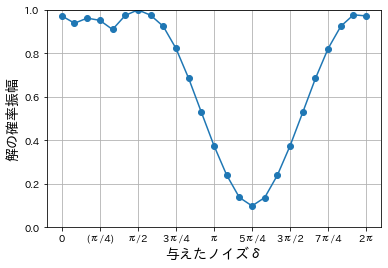
\includegraphics[width=70mm]{figures/sample.png}
\caption*{図 ノイズ$\delta_y$を加えた時の最適な繰り返し回数の推移}
\label{fig:P(k)}
\end{figure}

\bibliographystyle{junsrt}
\bibliography{references}
\end{document}